\chapter{Projektorganisation}

Bei der Organisation des Projektes wurde auf Microsofts Team-Data-Science-Prozess zurückgegriffen. Dieser ist optimiert für agile Entwicklung und passt, unter anderem durch den definierten Anfang und das definierte Ende, besser zu diesem Projekt als CRISP-DM. Die flexiblere Gestaltung des Arbeitsprozesses durch Abbildung der Interdependenzen der großen \glqq Überschriften\grqq\ des Projektlebenszyklus kam der Entwicklung ebenso zugute. Die Gestaltung des Arbeitsprozesses, vor allem mit weniger Erfahrung in diesem Bereich, wäre ohne häufigerem Wechsel zwischen den einzelnen Phasen nicht möglich gewesen.

Leider sind die Links zu TDSP, sowohl aus dem Studienscript, als auch von den referenzierenden GitHub-Seiten, auf Microsoft nicht mehr verfügbar. Das stattdessen angezeigte Dokument AI-Implementierung enthält zwar einen Verweis auf TDSP, zu dem Dokument selbst gelangt man jedoch nicht mehr. In diesem verhältnismäßig jungen Wirtschaftszweig folgen Weiterentwicklungen von Prozessen und Technologien Schlag auf Schlag.

Die Ordnerstruktur, die für die Organisation des Projektes angelegt wurde, orientiert sich an einer Azure TDSP Vorlage \citep{microsoft_azure_azure-tdsp-projecttemplate_2023}, die zusätzlich um den Überbau einer Ordnerstruktur für eine gesamte Softwareentwicklung ergänzt bzw. erweitert wurde. Das Projekt steht weiters mit der gesamten bisherigen Entwikclung auf GitHub unter dem Link 

\begin{center}\url{https://github.com/GGProjects/DLMDWME01}\end{center} 

zur Verfügung.

Die nachfolgende Abbildung zeigt die wesentlichen Elemente der bereitgestellten Ordnerstruktur. Auch wenn diese, in Teilen, für den Bedarf dieses Projektes zu umfangreich scheint, war die Intention, die Erstellung einer Vorlage für zukünftige Projekte zu schaffen, wo der Data Science Prozess in eine Softwareentwicklung eingebettet ist. Die einzelnen Modell- und Packageordner könnten auch als eigene Git-Repos angelegt werden. Die Nummerierung sorgt für gleichbleibende Anordnung und leicht zu verwaltende Strukturen.

\definecolor{mygray}{rgb}{0.9,0.9,0.9}
\lstset{backgroundcolor=\color{mygray},
	captionpos=b,  % sets the caption-position to bottom
	emph={}, 
	emphstyle=\color{red},
	basicstyle=\small,
	frame=single,
	framextopmargin=6pt,
	framexbottommargin=6pt,
	morecomment=[l][\color{red}]{/},}

\begin{figure}[h]
\caption{Struktur des Ordneraufbaus}
\begin{tabular}{c}  
\lstinputlisting[label=folder]{01_resources/tree.txt}
\end{tabular}\\
\centering
Quelle: Eigene Darstellung.
\label{tab:structure}
\end{figure}

\FloatBarrier

Die, in TDSP definierten Rollen und Aufgabenbereiche wurden, aufgrund der Projektgröße, nicht berücksichtigt, die benötigten Features waren gemäß Aufgabenstellung ebenso bereits vorgegeben. Der Use Case wurde in einem anderen Studiengangsmodul analysiert \citep{grunsky_rettungsdienst_2024}. An der Stelle hätte es sich auch angeboten User Stories für die Implementierung der Features abzuleiten. The Use Case Handbook \citep{microtool_gmbh_use_2017} stellt dafür eine wunderbare Unterstützung dar. Zu diesem Zeitpunkt des Projektes lag der Fokus jedoch auf dem Machine Learning Canvas \citep{dorard_machine_2022}, der ebenfalls eine gute Unterstützung in diesem Bereich bietet. Für zukünftige Projekte wurde jedenfalls mitgenommen, die beiden Ansätze zu kombinieren, um im Vorfeld bereits die bestmögliche Vorbereitung für eine Projektplanung und Umsetzung zu erreichen.

In den nachfolgenden Abschnitten dieser Arbeit wird auf die einzelnen Phasen des Lifecycle eingegangen, wobei sich die Struktur des Dokuments an der Vorlage eines Projektabschlussberichtes nach TDSP orientiert. \citep{microsoft_azure_azure-tdsp-projecttemplatedocsprojectexit_2023}

\begin{figure}[h]
\centering
\caption{Darstellung des Team Data Science Prozesses}
\includegraphics[width=15cm]{01_resources/tdsp.png}\\
Quelle: TDSP Data Science Lifecycle \citep{microsoft_azure_tdsp_2017}
\label{fig:tdsp}
\end{figure}

\FloatBarrier

\chapter{TDSP Projektabschlussbericht}

\section{Business Problem} 

Die Aufgabenstellung fokusiert auf einen klar abgegrenzten Aufgabenbereich innerhalb des  Berliner Rot Kreuz Rettungsdienstes, nämlich auf eine Vorhersage des Bedarfes an Bereitschaftspersonal für Einsatzfahrten. Das aktuelle Vorgehen sah, bis dato, eine fixe vorgehaltene Anzahl von 90 Bereitschaftseinsatzfahrer:innen für jeden Tag vor. Dieser Fixwert nimmt keine Rücksicht auf bestehende Saisonalitäten, eine Effizienzsteigerung soll daher durch einen Machine Learning Ansatz erzielt werden. 

Die, in den Projekt-Grundlagendokumenten abgelegte, Use Case Analyse \citep{grunsky_rettungsdienst_2024} versucht, durch Anwendung des Machine Learning Canvas zusätzliches Business Understanding aufzubauen. So wurde an dieser Stelle zum Beispiel eine Vorgabe des Projektes, nämlich die Bereitstellung der Vorhersage bis zum 15. Tag des Monats, abgeändert und bereits am 10. Tag des Monats verlangt. Auch wurden an dieser Stelle weitere Datenquellen diskutiert, die eine Forecast des benötigten Bereitschaftspersonals möglicherweise unterstützen und verfeinern könnten. Diese Features wurden im Projektplan jedoch auf eine niedrigere Priorität gestuft und könnten Verbesserungen für zukünftige Weiterentwicklungen darstellen. 

\section{Data Processing}
\label{dp}
Die Vorlage des TDSP Abschlussberichts stellt in diesem Punk, der im Prinzip der Phase Data Acquisition and Understanding entspricht, den originalen Datensatz im Vergleich zu dem, für das Modell, prozessierten Datensatz dar. Die Vorlage bezieht sich in diesem Punkt auf ein erstelltes Machine Learning Modell. Aus Sicht der, in diesem Modul, gewonnenen Erkenntnisse ist dieser Zugang unvollständig. 

Es wurden im Zuge dieser Arbeit ein Baseline-Model erstellt und zwei etwas ausgefeiltere Modelle. Die Vorgehensweise der ersten Erstellung einer Benchmark war nicht nur eine Vorgabe der Aufgabenstellung, sondern ist eine gängige Praxis. Auf dem Weg zu einem fortschrittlicheren Modell ist es sehr wahrscheinlich auf zusätzliche Ideen zu stoßen, Zwischenlösungen auszuprobieren oder einfach nur zwei vielversprechende Ansätze zu verfolgen ohne zu wissen, welcher davon sich als der Bessere entpuppt. Das Datenschema des originalen Datensatzes wird im Data Dictionary (Anhang \ref{app:dict}) dargestellt und in Anhang \ref{app:explore}, der explorativen Analyse, näher untersucht. 

Hierbei wurden mögliche Vorhersageansätze diskutiert, wobei zwei davon weiter verfolgt wurden. Die vorherzusagende Zielvariable ist dabei stets der tageweise Bedarf von Bereitschaftsfahrenden. Der erste Ansatz verfolgt dabei eine direkte Vorhersage der Zielvariablen auf Basis der eigenen Saisonalität. Im zweiten Ansatz wird die Korrelation der Zielvariablen zu den eingehenden Notrufen genutzt. Letztere sind für eine Vorhersage durch eine saisonale Modellierung besser geeignet. Die Datenschemata, die für die einzelnen Modelle verwendet wurden, weichen geringfügig von einander ab. Sample-Daten der einzelnen Modelle wurden im Rahmen der Modellentwicklung in der Ordnerstruktur hinterlegt. In der zukünftigen Arbeit mit einer Datenvorhersage werden die Tagesdaten gemäß dem Eingangsdatenschema weiterhin durch die Planungsstelle des Bereitschaftsdienstes elektronisch eingegeben. Diese werden als Grundlage für neuerliche Trainings und Vorhersagen genutzt. Diese Rohdaten werden jedoch nicht unmittelbar nach der Eingabe prozessiert, sondern erst bei der Vorhersage. Das ermöglicht eine einfache Implementierung neuer Modelle ohne Änderung der Basisdaten.

Eine Erweiterung der Datengrundlage wurde in der Use Case Analyse erläutert. Die Idee dabei war es, die vorliegenden Unternehmensdaten des Roten Kreuzes mit weiteren Daten anzureichern um diese als Prädiktoren für eine Vorhersage der benötigten Bereichtschaftsfahrer:innen zu verwenden. Im konkreten ging es dabei um eine Einbeziehung von Wetterdaten, insbesondere Wettereignisse wie zB Schneefall oder überdurchschnittliche Hitze, Wochenend- und Feiertage, sowie Daten geplanter Veranstaltungen im Raum Berlin. Eine Untersuchung dieser Daten auf Tauglichkeit als Prädiktoren wäre in einer Fortsetzung des Projektes zur Verbesserung des Modelles denkbar.


\subsection{Data Understanding}
\label{du}

Der bereitgestellte Datensatz mit Messwerten des Einsatzfahrdienstes erstreckt sich über einen Zeitraum von etwa drei Jahren (von 01.04.2016 bis 27.05.2019) und enthält 1152 Datenpunkte zu je acht Merkmalen.

%\FloatBarrier

%\vspace{1em}

\begin{table}[h]
\centering
\caption{Struktur der vorhandenen Daten}
\begin{tabular}{|c|c|c|c|}
\hline 
\textbf{Variable} & \textbf{Datentyp} & \textbf{Beschreibung} \\ 
\hline 
...1 & Numeric (double) & Zähler  \\ 
\hline 
date & Date (\%Y-\%m-\%d) & Datum  \\ 
\hline 
n\_sick & Numeric (double) & Anzahl erkrannkte Einsatzfaher:innen  \\ 
\hline 
calls & Numeric (double) & Anzahl der Notrufe  \\ 
\hline 
n\_duty & Numeric (double) & Anzahl Einsatzfahrer:innen im Dienst \\ 
\hline 
n\_sby & Numeric (double) & Anzahl verfügbares StandBy Personal  \\ 
\hline 
\colorbox{hellrot}{sby\_need} & Numeric (double) & Anzahl aktiviertes StandBy Personal, \colorbox{hellrot}{Zielvariable}  \\ 
\hline 
dafted & Numeric (double) & Zusätzlich aktiviertes Personal, da sby\_need zu niedrig  \\ 
\hline 
\end{tabular} 
\label{tab:data}
\end{table}
\FloatBarrier
%\vspace{1em}

Die erste Spalte (\textit{id}), die bisher konstante Einteilung des Bereitschaftspersonals (\textit{n\_sby}), sowie die Anzahl der zusätzlich benötigten Fahrer:innen (\textit{dafted}) wurden gleich zu Beginn wieder entfernt und die Daten in Tageszeitreihendaten konvertiert. Das Datum dient dabei als Schlüssel zur eindeutigen Identifikation des Datenpunktes. 

\begin{figure}[h]
\centering
\caption{Zeitlicher Verlauf der Zielvariablen}
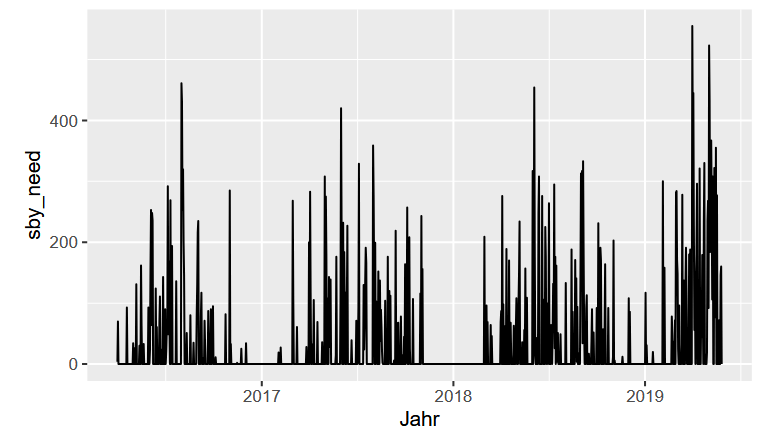
\includegraphics[width=15cm]{01_resources/timeplot_sby_need.png}\\
Quelle: Eigene Darstellung.
\label{fig:timeplot}
\end{figure}

\FloatBarrier

Die vermutete Saisonalität ist in der zeitlichen Darstellung des Bedarfs an Bereitschaftsfahrenden gut erkennbar. Augenscheinlich scheint es monatliche Spitzen in der Zielvariablen zu geben und um den Jahreswechsel ist oft nur  geringer Bedarf vorhanden. Mit dem Jahreswechsel auf 2019 ändert sich das Muster der Bedarf weist ab diesem Zeitpunkt deutlich höhere Spitzen auf. Weiters werden auch die raschen Wechsel zwischen wenig bis kein Bedarf und sehr hoher Bedarf in der Darstellung deutlich. Diese Volatilität verlangt eine überlegte Generalisierung des Modells und einen klar definierten Fokus der Vorhersage. Gemäß Aufgabenstellung ist dieser auf eine Abdeckung der Spitzenwerte ausgerichtet.

Die Korrelation zwischen der Zielvariablen und dem Merkmal der eingegangenen Notrufe wurde bereits angesprochen. Die unten angeführte Grafik macht den, nahezu linearen, Zuammenhang anschaulich.

Die Abstände im augenscheinlichen Intercept (dem Schnittpunkt mit der x-Achse) betragen zwischen den Jahren jeweils etwa 500 Notrufe. Das ist jeweils das fünffache des jährlichen Anstiegs von diensthabendem Personal. Von 2018 auf 2019 wurde das diensthabende Personal nicht erhöht, weswegen auch im Intercept der linearen Korrelation keine Veränderung erkennbar ist. Wurden weniger Anrufe als der jeweilige Intercept getätigt wurde auch kein Bereitschaftspersonal aktiviert. 

\begin{figure}[h]
\centering
\caption{Korrelation der Zielvariable zu den Notrufen}
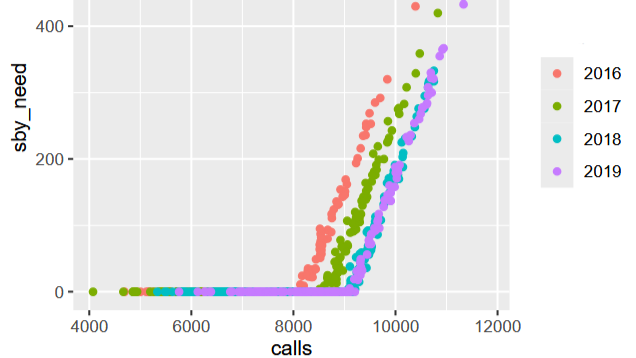
\includegraphics[width=15cm]{01_resources/call_correlation_year.png}\\
Quelle: Eigene Darstellung.
\label{fig:call_correlation_year}
\end{figure}
\FloatBarrier

Die, auf der Shannon Entropy basierende, spektrale Entropy liefert eine erste Aussage über die Verteilung und Vorhersagbarkeit von Zeitreihendaten. Im vorliegenden Datensatz wurde der beste Entropy-Wert für den gleitenden Durchschnitt der eingehenden Notrufe erzielt. Dieser wird im nachfolgenden jährlichen Saisonalitätsplot dargesellt. Die, in den Daten auftretenden, Muster sind hier gut erkennbar, genauso wie ein augenscheinlicher Aufwärtstrend über die Jahre.

\begin{figure}[h]
\centering
\caption{Verteilung der Notrufe nach Jahr}
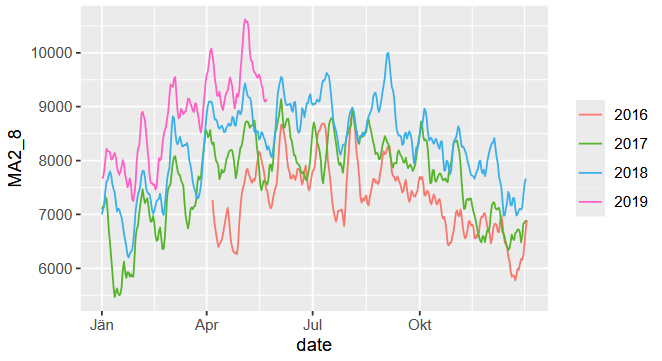
\includegraphics[width=15cm]{01_resources/calls_year.png}\\
Quelle: Eigene Darstellung.
\label{fig:callsperyear}
\end{figure}
\FloatBarrier

Die beschriebene Korrelation der Zielvariable zu den eingegangenen Notrufen (unter Berücksichtigung des diensthabenden Personals) sowie die besser modellierbare Saisonalität der eingegangenen Notrufe dienten als Grundlage für die Entwicklung fortschrittlicherer Modelle.

\section{Modeling}

Die Entwicklung der Modelle wurde mir der Programmiersprache R umgesetzt. Besonders hilfreich war hierbei das online Buch sowie das dazugehörige R Package \glqq Forecasting Principles and Practice\grqq\ \citep{hyndman_forecasting_2021}. Für die Entwicklung der Modelle wurden, wie bereits beschrieben, zwei Ansätze gewählt.  Im Vordergrund stand dabei stets die Anforderung, nie zu wenig Bereitschaftspersonal vorherzusagen. Gerade bei den vorliegenden, sehr stark und abrupt schwankenden Eingangsdaten der Zielvariablen, ist die Herausforderung, dass man zwischen Kosteneffizienz und Abdeckung der Maximalbedarfsspitzen wählen muss.  

In der explorativen Datenanalyse (Anhang \ref{app:explore}) wurde festgehalten, dass 35 Personen in Bereitschaft für Tage mit niedrigem Bedarf einen guten Durchschnittswert bilden. Die Einteilung von null Personen in Bereitschaft scheint geschäftsseitig unrealistisch, der Minimalwert wird daher für alle Modelle mit 35 Personen festgelegt.

 \subsection{Baseline Model} 

Das Baseline-Model (Anhang \ref{app:baseline}) wird direkt anhand der Saisonalität der Zielvariablen trainiert und verwendet dabei ein Lineares Model für Zeitreihen (TSLM), das auch ebenso Trends und saisonale Muster abbilden kann. Um eine ausreichende Generalisierung zu erreichen und die Vorhersage zuverlässiger zu machen, wurden die Daten mit einer, über sieben Tage, gleitenden 99\% Quantille  geglättet und anschließend zu wöchentlichen Daten aggregiert. Bei der Aggregation wurden die jeweiligen Maxima der gleitenden Quantille als Wochenwert herangezogen. Nach der Vorhersage, werden die Wochendaten wieder in Tagesdaten (gem. Anforderung) aufgetrennt, wobei die Tage einer Woche entsprechend immer denselben Wert aufweisen. Die Bedarfsspitzen werden durch dieses Model nicht korrekt vorhergesagt, die Saisonalität wird jedoch modelliert. In der Darstellung werden die Vorhersagen (blau) den Daten des Testdatensatzes (schwarz), über einen Zeitraum von zwei Monaten, gegenübergestellt. Des Weiteren werden für die Vorhersage auch die 80\%, 90\% und 99\% Konfidenzintervalle angezeigt.

\begin{figure}[h]
\centering
\caption{Vorhersage des Basline-Models}
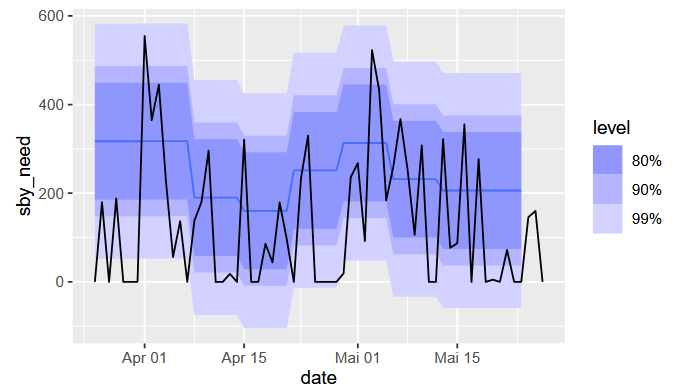
\includegraphics[width=15cm]{01_resources/baseline_prediction.png}\\
Quelle: Eigene Darstellung.
\label{fig:baseline}
\end{figure}

\FloatBarrier

Für die spätere Evaluierung wurde, als zweites Baseline-Model, auch das aktuelle Vorgehen mit einem Fixwert von 90 Bereitschaftsfahrenden mit aufgenommen.

 \subsection{Advanced Model} 

Das Advanced-Model (Anhang \ref{app:adv}) basiert auf dem Modell \glqq Seasonal and Trend decomposition using Loess\grqq\ (STL). Dieser Algorithmus wurde bereits in der explorativen Datenanalyse (Anhang \ref{app:explore}) verwendet um die saisonalen Komponeten der eingehenden Notrufe auf Basis eines gleitenden Durchschnitts zu untersuchen. Dabei werden die Daten in den Trend, verschiedene Saisonalitäten und den \glqq Remainder\grqq\ (den Rest) aufgesplittet. So können saisonale Muster in den Daten gut erkannt, analysiert und beschrieben werden. In diesem Ansatz wird jedoch nicht die Zielvariable direkt vorhergsagt sondern die, schöner modellierbare, Saisonalität der eingehenden Notrufe. Für die weitere Vorhersage des Bedarfs an Bereitschaftspersonal wird die beschriebene lineare Korrelation zwischen den eingehenden Notrufen und dem StandBy-Bedarf genutzt. Diese wurde durch ein einfaches lineares Modell abgebildet.

Die, in Punkt \ref{du} Data Understanding,  festgestellte Auswirkung der jährlichen Erhöhung des diensthabenden Personals mit einem Faktor 5 auf den Intercept der Korrelation wird im linearen Modell berücksichtigt. Bei der Anwendung des Modells muss daher die Anzahl des diensthabenden Personals als Parameter mitgegeben werden.

\[modifizierte Notrufe_t = Notrufe_t - Korrekturwert_t\ \ |\ \   Korrekturwert_t = (n\_duty_{year} - 1700) * 5\]

Der Intercept wird nach Korrektur fix auf 8150 gesetzt. Werden weniger Notrufe vorhergesagt wird durch das Model der fixierte Minimalwert von 35 Personen in Bereitschaft ausgegeben.  Die u.a. Grafik zeigt die modifizierte lineare Abhängigkeit zwischen den eingehenden Notrufen und dem StandBy Bedarf mit dem fixen Intercept bei 8150.


\begin{figure}[h]
\centering
\caption{Korrelation modifizierter Notrufdaten mit der Zielvariablen}
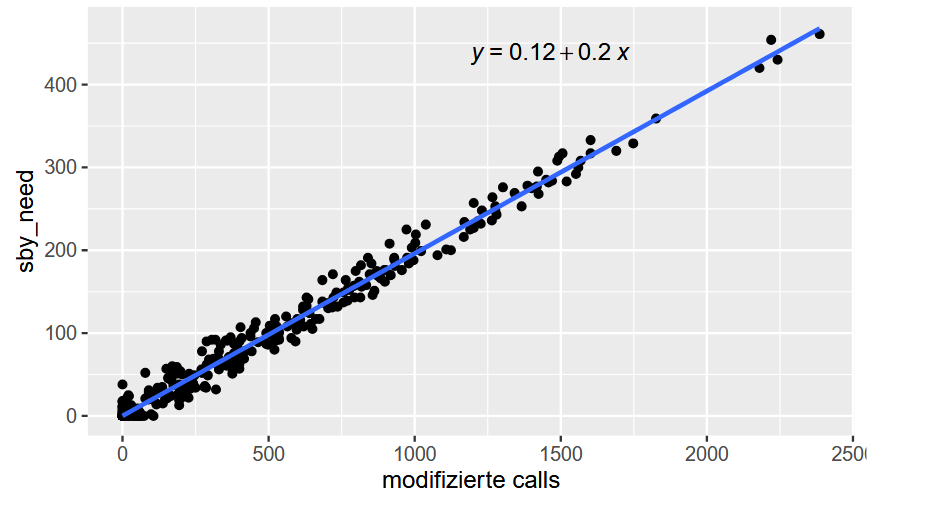
\includegraphics[width=15cm]{01_resources/reg_call_correlation_year.png}\\
Quelle: Eigene Darstellung.
\label{fig:regcall-corr-year}
\end{figure}
\FloatBarrier

Der STL Algorithmus erkennt zwar die Spitzenaufkommen in den eingehenden Notrufen, im Vergleich mit dem Testdatensatz wurden diese allerdings oft wenige Tage verschoben prognostiziert. Die, allgemein fehlende, Generalisierung der Vorhersage wird durch Anwendung eines gleitenden Maximums  auf die Prognose erreicht. 

Das Advanced Model wurde in zwei Varianten evaluiert. In den finalen Programmcode wurde allerdings nur die Version 2 aufgenommen. Der Unterschied der beiden Modelle liegt in der Fenstergröße des gleitenden Maximums und (in der Version 2) einer Reduktion des Parameters \glqq diensthabendes Personal\grqq\ um einen Wert von 100. Durch die Modifikation dieses Parameters kann die Höhe des vorhergesagten Bedarfs beeinflusst werden.

\begin{figure}[h]
\centering
\caption{Vorhersage Advanced Model V2}
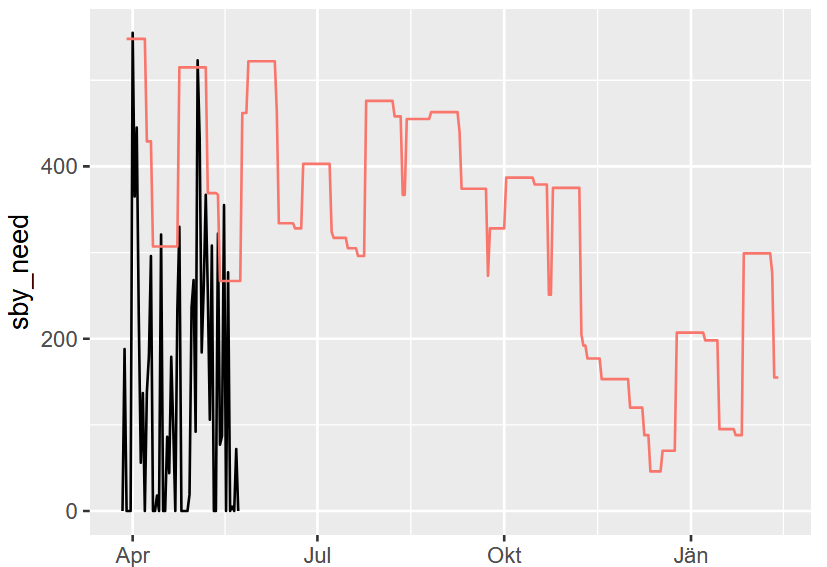
\includegraphics[width=15cm]{01_resources/adv2.png}\\
Quelle: Eigene Darstellung.
\label{fig:adv2}
\end{figure}
\FloatBarrier

Die Darstellung zeigt die Ausgabe der Vorhersage (rot) über den Zeitraum von elf Monaten. Die Werte des Testdatensatzes (schwarz) sind nur in den ersten beiden Monaten der Prognose vorhanden. Die jährliche und monatliche Saisonalität werden von dem Modell gut aufgenommen. Durch die stark ausgeprägte Generalisierung wird jedoch überwiegend eine deutlich zu hohe Anzahl an Bereitschaftspersonal vorgesehen.


 \subsection{Prophet Model} 

In der Use Case Analyse wurde der Algorithmus \glqq Facebook Prophet\grqq\ als möglicherweise passender Ansatz für die gegenständliche Machine Learning Aufgabe recherchiert. Dieser Algorithmus wurde für Zeitreihenvorhersagen entwickelt und verwendet dabei ein zusammengesetztes Modell aus Trend, Saisonalität und speziellen Ereignissen in Zeitreihen. \citep{taylor_forecasting_2017}. Der Vorteil von Facebook Prophet, oder kurz \textit{Prophet}, liegt darin, dass in einer möglichen, zukünftigen Weiterentwicklung des Modells auch Tage mit besonderen Ereignissen, wie zB Veranstaltungen und speziellen Wetterverhältnissen, mit modelliert werden können. Diese würden dann a priori in eine Vorhersage miteinbezogen und in der Prognose berücksichtigt werden.

Im Advanced-Modell wurde versucht einen Puffer für die Spitzenwerte anhand eines gleitenden Maximums über die vorhergesagten Notrufe zu erreichen. Bei Prophet erscheint die Verwendung von Konfidenzintervallen möglich. Daher wird in diesem Ansatz der Puffer durch Verwendung der 90\% Quantille als Vorhersagewert erreicht. Das Schöne hierbei ist, dass der zu verwendende Prozentsatz für die Berechnung im codierten Modell als Hyperparameter gesetzt werden kann. Wie auch im Advanced Modell V2 wird, zum Vergleich der Ergebnisse, die Höhe des diensthabenden Personals um 100 reduziert. Damit wird die Anzahl des vorhergesagten Bereitschaftspersonals etwas angehoben. 
 
\begin{figure}[h]
\centering
\caption{Vorhersage Prophet Model}
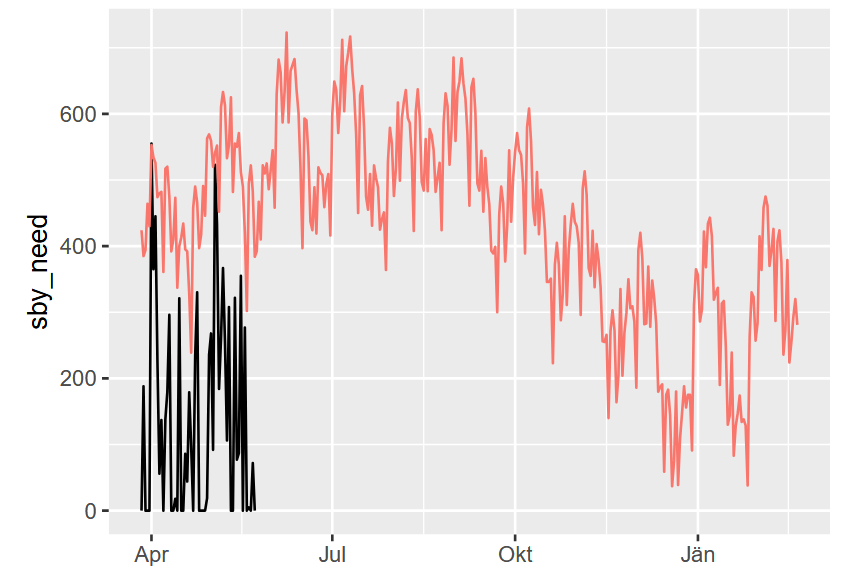
\includegraphics[width=15cm]{01_resources/prophet.png}\\
Quelle: Eigene Darstellung.
\label{fig:prophet}
\end{figure}
\FloatBarrier 

Die Darstellung zeigt wiederum die Ausgabe der Vorhersage (rot) über den Zeitraum von elf Monaten mit gleichzeitiger Anzeige der Testdaten (schwarz) für die ersten beiden Monate der Prognose. Bei Anwendung dieses Modells sind die einzelnen Komponenten der Saisonalität in der Vorhersage zu erkennen. Man sieht sowohl den jährlichen Verlauf mit einem Abfall des Bedarfs bis zum Jahreswechsel, als auch ein augenscheinlich relativ fixes Muster in den Monatsdaten. Der Grad der Flexibilität in den saisonalen Mustern kann in Prophet durch Hyperparameter gesteuert werden. In diesem Bereich bietet Prophet auch die meisten Möglichkeiten das Modell noch feiner zu \glqq tunen\grqq\ . Das Machine Learning Framework \textit{Caret} \citep{kuhn_caret_2019} bietet Unterstützung im Finetuning durch ein automatisieretes \glqq Durchtesten\grqq\ mehrerer Kombinationen an Hyperparametern. Das war in dem, hier verwendeten, Package \textit{fpp3} \citep{hyndman_forecasting_2021} nicht möglich, dafür ist dieses speziell für die Arbeit mit Zeitreihen entwickelt. In einer Weiterentwicklung des gegebenen Anwendungsfalles wäre ein Hyperparameter-Finetuning für den Prophet-Ansatz jedenfalls zielführend. 

Dank Verwendung der 90\% Quantille für die Prognose, wird auch bei diesem Modell überwiegend eine zu hohe Anzahl an Bereitschaftspersonal vorgesehen. Die Höhe der Vorhersage ist, wie auch beim Advanced Model, über gesetzte Parameter beeinflussbar und sollte mit den Entscheidungsträgern noch diskutiert werden.

\newpage 

\subsection{Modellresultate} 

\begin{table}[h]
\centering
\caption{Vergleich der ML-Modelle}
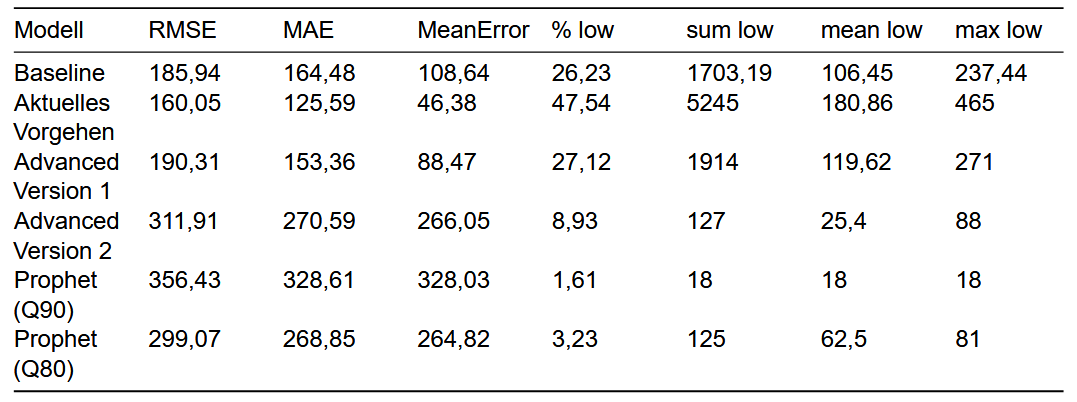
\includegraphics[width=15cm]{01\_resources/modellvergleich.png}\\
Quelle: Eigene Darstellung.
\label{tab:modeleval}
\end{table}
\FloatBarrier 

Die angeführte Tabelle zeigt einen Vergleich der beschriebenen Modelle (inklusive des aktuellen Vorgehens) anhand unterschiedlicher Messwerte. Diese sind folgendermaßen zu interpretieren:

\begin{itemize}
 \itemsep-8pt
 \item \textbf{RMSE}: Gängiger Messwert. Berechnet die Wurzel der mittleren quadrierten Abweichung
 \item \textbf{MAE}: Gängiger Messwert. Berechnet die durchschnittliche absolute Abweichung
 \item \textbf{MeanError}: Die durchschnittliche Abweichung. Positive Werte deuten auf eine durchschnittliche Überschätzung durch das Modell hin
 \item \textbf{\% low}: Prozentanteil der Vorhersagen, wo das Modell zu niedrig geschätzt hat
 \item \textbf{sum low}: Die Summe zu niedrig geschätzten Personals, gleichzeitig Personal, das zusätzlich hätte aktiviert werden müssen.
 \item \textbf{mean low}: Der Durchschnitt jener Schätzungen, die unter dem Bedarf lagen. 
 \item \textbf{max low}: Die maximale Abweichung jener Schätzungen, die unter dem Bedarf lagen.
 \end{itemize}


Die, in der obigen Tabelle, dargestellten Messwerte beziehen sich auf eine Gütebewertung der Modelle in einem Testzeitraum von zwei Monaten. Hierbei wird ersichtlich, dass beim bisherigen Vorgehen etwa bei der Hälfte der Tage zu wenig Bereitschaftspersonal vorgesehen wurde. In den zwei Monaten Testzeitraum hätten in Summe 5245 zusätzliche Bereitschaftsfahrer:innen aktiviert werden müssen. Hinsichtlich einer durchschnittlichen Abweichung (RMSE, MAE oder MeanError) schneidet das aktuelle Vorgehen jedoch am Besten ab. Eine erste Verbesserung in Bezug auf Unterschätzungen des Bedarfs an Bereitschaftspersonal zeigen das Baseline Modell und das Advanced Modell in der Version 1. Die beiden Modelle liefern ähnliche Messwerte und schaffen es Unterschätzungen auf ein Viertel der Vorhersagen zu senken, wohingegen RMSE und MAE noch mit dem aktuellen Vorgehen vergleichbar bleiben. Das Advanced Modell in Version 2, sowie zwei Varianten des Prophet Modells (einmal mit 80\% Konfidenzintervall und einmal mit 90\% Konfidenzintervall) steigen bei RMSE und MAE deutlich in die Höhe, was sich, im Gegenzug, in einer ebenso deutlichen Verringerung der Fälle von Unterschätzung widerspiegelt. 

Auf welches Modell, die Entscheidung schlussendlich fällt ist abzuwägen und wird mit den Entscheidungsträgern diskutiert werden müssen. Durch \glqq Finetuning\grqq\ von Hyperparametern ist gegebenenfalls noch eine Verbesserung einzelner Modelle zu erreichen. Derzeit sind die Modelle \glqq Baseline\grqq\ , \glqq Advanced V2\grqq\ und \glqq Prophet Q90\grqq\ ausprogrammiert.

Für alle Modelle ist die Rechendauer als sehr positiv zu bewerten. Die Zeiten für Training und Vorhersage betrugen, in der Entwicklung, beim Baseline Modell in Summe 0,28 Sekunden, bei den Advanced Modellen in Summe 0,97 Sekunden und den Prophet Modellen in Summe 13,60 Sekunden. Für die Entwicklung wurde ein Notebook vom Typ Dell Latitude 5490, Intel i7 vPro (8th Gerneration) mit 16 Gb RAM (aus dem Jahr 2018) verwendet. Für eine Umsetzung der modellbasierten Vohersage im Bereitschaftsdienst ist daher nicht mit großen Anschaffungskosten hinsichtlich Hardwarekapazitäten zu rechnen.

\subsubsection{Fehleranalyse} 
Die Schwachsellen der vorgestellten Modelle, liegen, wie bereits im Vergleich erkennbar, in der Unfähigkeit sowohl niedrigen als auch hohen Bedarf korrekt vorherzusagen. Hier wird eine Entscheidung getroffen werden müssen, worauf der Fokus liegen soll. Eine korrekte Vorhersage von Tagen mit niedrigem Bedarf spart Bereitschaftskosten, wohingegen der Einsatz von zu wenig Bereitschaftsfahrenden möglicherweise einen Reputationsschaden nach sich ziehen kann. 
An dieser Stelle wäre es hilfreich mit den Entscheidungsträgern gemeinsam eine Use Case spezifische Kostenfunktion für die Bewertung der Modelle zu entwerfen. Diese kann dann die tatsächlichen Kosten der Vorhersage ermitteln. 

Weiters ist es für Modelle des maschinellen Lernens schwierig, allgemeine Änderungen im Muster der Daten (Datendrift) abzubilden. Beim vorliegenden Datensatz ist mit dem Jahreswechsel 2018/2019 eine solche Änderung erkennbar. Diese fällt in einen Zeitraum, der bereits die Testdaten für die Gütebewertung der Modelle beinhalten und daher nicht für das Training herangezogen werden sollte. Das Sammeln weiterer Trainingsdaten, die das Aufkommen nach 2019 beschreiben könnte die Modellgüte maßgeblich verbessern. Bei den vorgestellten Modellen, ist der Prophet Algorithmus auch in der Lage, vorgegebene \textit{Changepoints} für Änderungen im Trend zu berücksichtigen. So könnten zB auch maßgebliche Trendwenden wie COVID-19 modelliert werden.

\section{Solution Architecture}

Die Implementierung des Vorhersagemodells in die tägliche Arbeit der Planungsstelle könnte dermaßen erfolgen, dass die Mitarbeitenden weiterhin täglich die Betriebsmetriken (wie auch im vorliegenden Datensatz), über ein Formular festhalten. Dieses kann, wie in der unteren Grafik dargestellt auch in Form einer Web-Applikation bereitgestellt werden.

Am 10. Tag jedes Monats wird über eine weitere Seite der Web-Applikation das Training und die Vorhersage für einen angegebenen Zeitraum (zB zwei Monate) angestoßen und die Mitarbeiter:innen erhalten die prognostizierten Werte als Liste und grafisch ausgegeben.

\begin{landscape}
\centering
\captionof{figure}{mögliches Dateneingabe-GUI} 
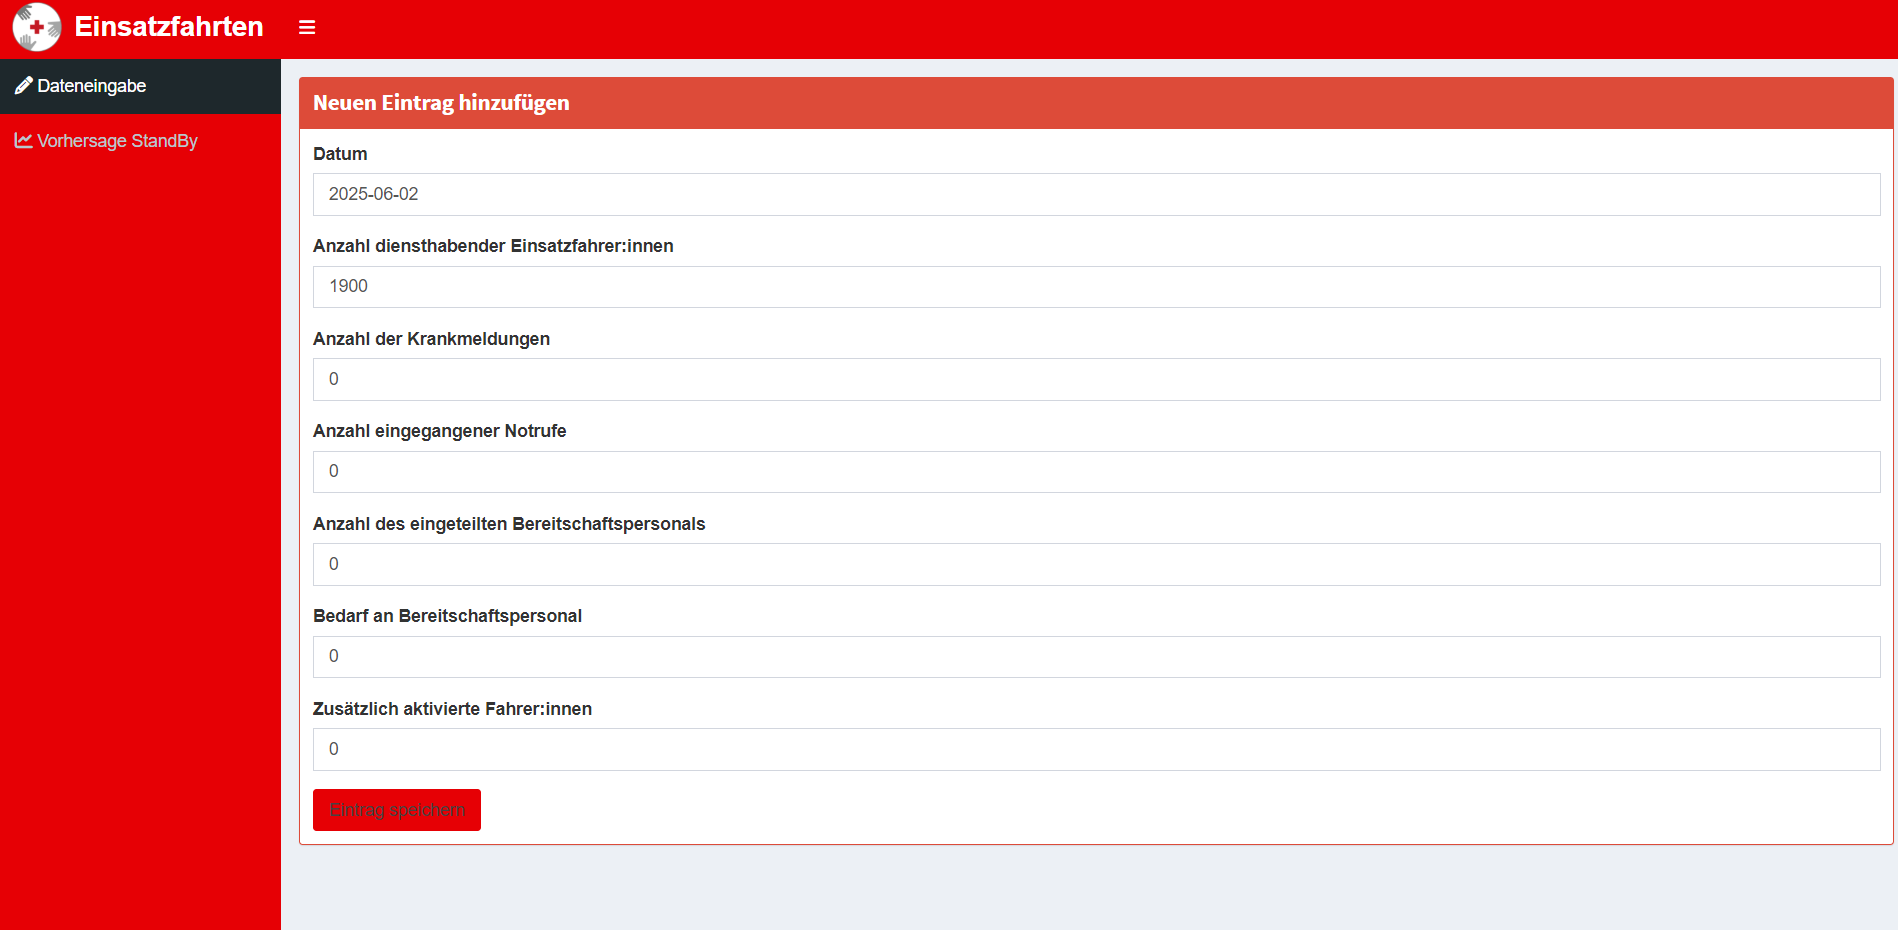
\includegraphics[width=22cm]{01_resources/dataentry.png}\\
Quelle: Eigene Darstellung.
\label{fig:dataentry}
\end{landscape}
\FloatBarrier 
  
\begin{landscape}
\centering
\captionof{figure}{mögliches Datenausgabe-GUI} 
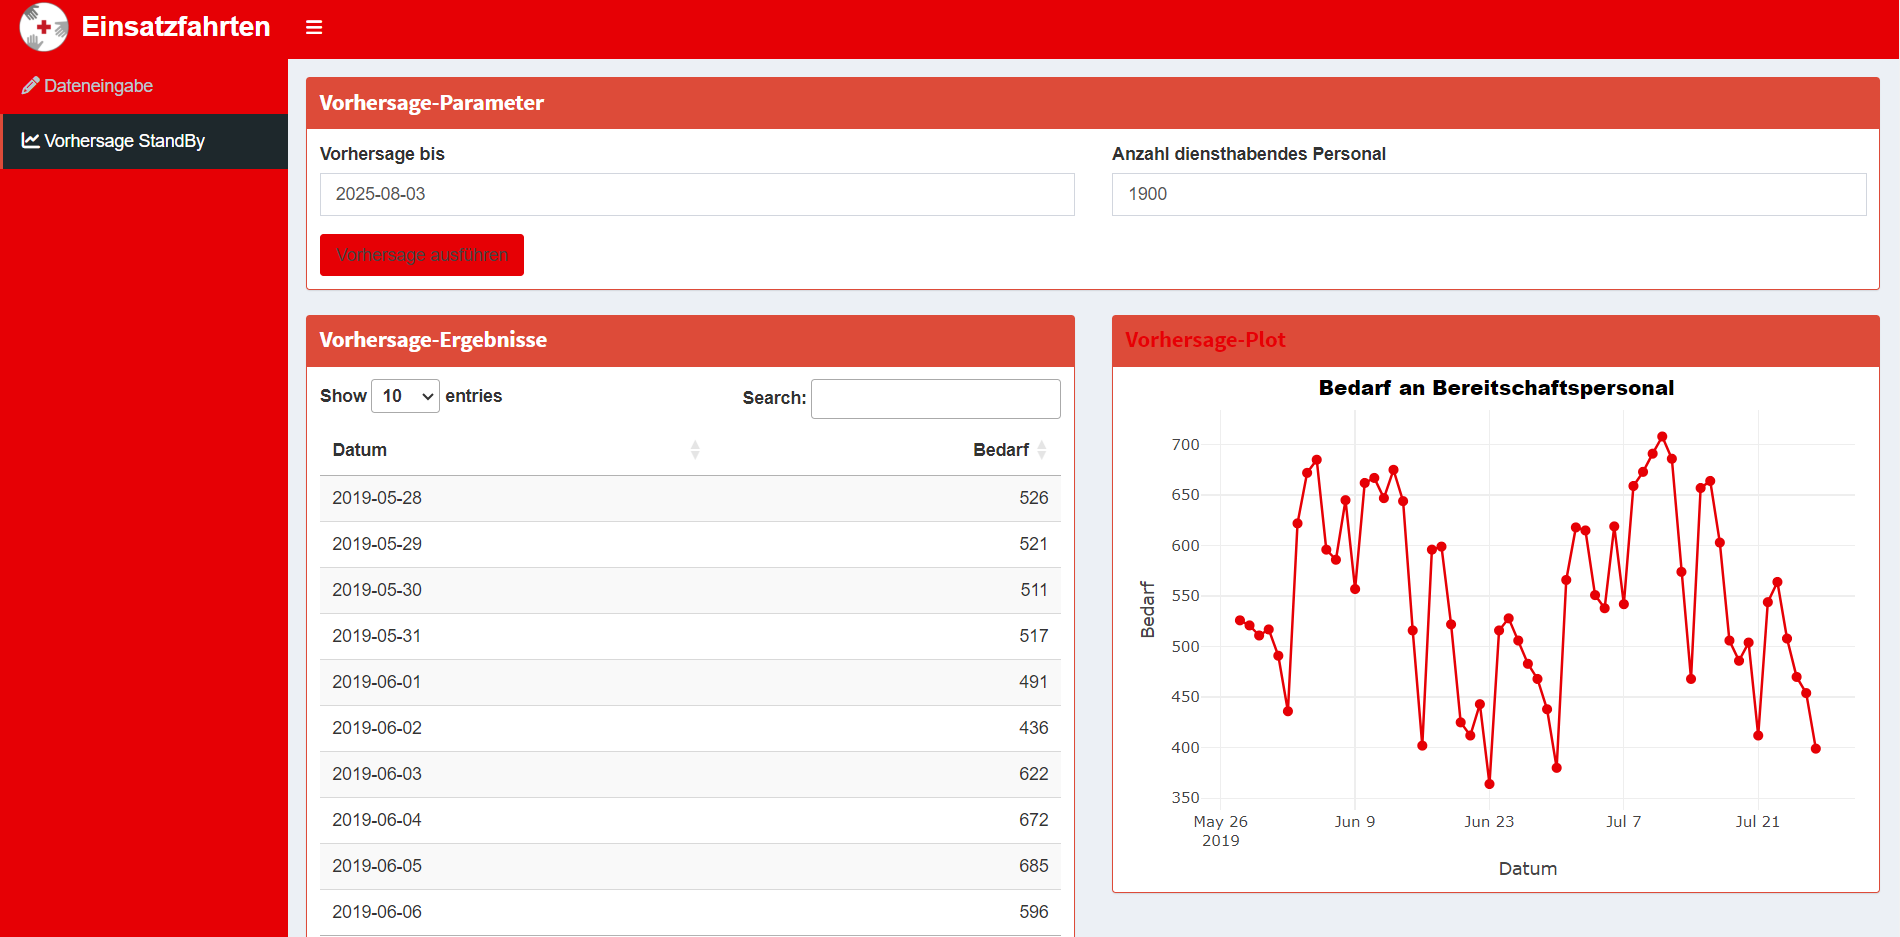
\includegraphics[width=22cm]{01_resources/dataforecast.png}\\
Quelle: Eigene Darstellung.
\label{fig:forecast}
\end{landscape}
\FloatBarrier
 
Die Planungsstelle hat nun noch weitere fünf Tage Zeit, diese Werte 

 \begin{enumerate}
  \itemsep-8pt
   \item	auf Plausibilität zu prüfen und eigene Erfahrung mit einfließen zu lassen. Prognostizierte Werte dürfen vom Personal der Planungsstelle abgeändert werden, das Bedarf allerdings klaren Regeln und einer hinreichenden Dokumentation, wie in Punkt Customer Acceptance (\ref{ca}) noch erläutert wird.
   \item mit Namen von Bereitschaftspersonal zu hinterlegen und so einen Bereitschaftsdienstplan zu erstellen.
 \end{enumerate}
 
Das Format der Ausgabe durch die Web-Applikation kann noch den Wünschen Planungspersonals angepasst werden. Zur nachvollziehbaren Modellbewertung sollte die Prognose nicht veränderbar (read-only) gespeichert werden. Abänderungen durch die Planungsstelle müssen gesondert dokumentiert und abgelegt werden.

Die derzeit im Repository verfügbare Web-Applikation bildet die Grundfunktionalität des beschriebenen Ablaufes dar. Dennoch sind hier noch einige Weiterentwicklungen und Verbesserungen für einen Betrieb vorzusehen. Hierzu gehören zum Beispiel die Änderung und Bearbeitung bereits angelegter \glqq Betriebsmetriken\grqq\ , oder auch die angesprochene Speicherung und Dokumentation von Prognosemodifikationen durch die Planungsstelle. Weiters wäre es sinnvoll, zusätzlich zu Training und Vorhersage, auch einen Trainings- und Testlauf, mit allen verfügbaren Modellen, anhand der gespeicherten historischen Daten durchführen zu können (zB durch Aktivieren einer Check-Box) und die Modellbewertungen analog zu Tabelle (\ref{tab:modeleval}), oder mit eigener Kostenfunktion, anzeigen lassen zu können. So kann in periodischen Abständen überprüft werden ob die Vorhersagealgorithmen in einem zuverlässigen Rahmen arbeiten, oder ob sich die Güte einzlner Modelle (zB aufgrund eines Datendrifts) verschlechtert.

Die Auswahl des anzuwendenden Vorhersagemodells wurde in der Web-Applikation bewusst weggelassen. Die Mitarbeitenden der Planungsstelle sollen sich nicht damit beschäftigen müssen, welches Modell, wie funktioniert und auch nicht begründen, warum sie welches Modell gewählt haben. Es wäre jedoch keine Schwierigkeit ein solches Feature in die Applikation zu implementieren, da beim Training derzeit das Prophet Modell standardmäßig beim Funktionsaufruf als Parameter mitgegeben wird, die Funktion aber so gestaltet ist, dass durch Veränderung dieses Parameters jedes implementierte Modell gewählt werden kann. 

Für die Implementierung neuer Modelle ist demnach auch einfach nur der Code für das Modell, analog zur Struktur und Namenskonvention bestehender Modelle im Ordner \textit{04a\_model\_standby\\03\_deployment} abzulegen und in der Applikation mit dem Parameter des Modellnamens aufzurufen. Sollten neue Modelle weitere zusätzliche Hyperparameter benötigen sind diese jedoch applikationsweit zu ergänzen.

Die, diesem Projekt vorangegangene, Use Case Analyse sieht für die geschäftszentrierte Messung des Erfolgs ein Monitoring der Vorhersagemodelle anhand von zwei Key Result Indikatoren (KRI) vor. Diese sind zwar nicht ausschließlich von der Arbeit der Vorhersage abhängig, spiegeln jedoch die Messung des, durch Implementierung der Modelle, gewünschten Effekts wider. Die beiden Werte werden in der Use Case Analyse \citep{grunsky_rettungsdienst_2024} wie folgt beschrieben:

\begin{itemize}
 \itemsep-8pt
 \item Eine statistisch aufbereitete Messung der „time-to-target“ , also der Zeit vom Anruf bis zum Eintreffen am Einsatzort bzw. der „no-shows“ , das sind Notrufe, die nicht bedient werden konnten. Natürlich hängen diese Werte von viel mehr Faktoren ab, als den verfügbaren Bereitschaftsfahrer:innen. Die Vermeidung von Totalausfällen (no-shows) aufgrund mangelnden Bereitschaftspersonals wird aber eine wesentliche Ziffer für den Erfolg des Modells darstellen.
 \item  Die mittleren Personalkosten pro Notruf sollten mit einer akkuraten Planung der Bereitschaftsfahrenden eigentlich abnehmen. Wenn man den o.a. Wert als K.O.-Kriterium für die Modellbewertung erachtet, so sagt dieser Wert (im Vergleich mit Vorangegangenen) aus, wie präzise das Modell arbeitet.
\end{itemize}

In der Use Case Analyse wurde davon ausgegangen, dass ein Vorhersagemodell sowohl niedrigen als auch erhöhten Bedarf korrekt vorhersagen würde. Die Modellentwicklung hat hier bis dato etwas anderes ergeben. Aus aktueller Sicht scheinen die beiden angeführten KRIs  für das Monitoring des Modells im gegenständlichen Anwendungsfall trotzdem Gültigkeit zu besitzen und könnten noch zusätzlich in die Applikation mit aufgenommen werden. In diesem Fall müsste nur noch die Frage geklärt werden, wer für die Dokumentation der erforderlichen Metriken verantwortlich ist.


\section{Benefits}
\label{ca}
Sowohl im Rahmen der Use Case Analyse \citep{grunsky_rettungsdienst_2024} als auch der Projektplanung \citep{grunsky_rettungsdienst_2025} wurden die Stakeholder des Projektes beleuchtet.  

Den \textbf{Bereitschaftsfahrenden} kommt der eine erfolgreiche Umsetzung des Vorhersagemodells zugute. Durch eine ausreichende Abdeckung werden kurzfristige Anrufe, ob man nicht evtl. doch Dienst versehen kann vermieden und die persönliche Freizeit dadurch planbarer. 

Für den \textbf{Rettungsdienst} bedeutet eine erfolgreiche Umsetzung möglicherweise eine Kostenersparnis, wenn geringerer Bedarf korrekt vorhergesagt würde, aber in jedem Fall die Vermeidung eines Reputationsschadens aufgrund mangelden Bereitschaftspersonals.

Die \textbf{Planungsstelle} sieht sich im täglichen Betrieb sogar mit zusätzlichem Aufwand und größerer Verantwortung konfrontiert. Dank des Vorhersagemodells wird nun nicht mehr, wie bisher, ein vorgegebener Tages-Fixwert angenommen sondern der von einem Sysem ermittelte wahrscheinliche Bedarf an Bereitschaftspersonal. Die Mitarbeiter:innen der Planungsstelle können diesen Wert nun übernehmen oder dokumentiert und begründet Abändern. In jedem Fall übernehmen Sie, anders als bisher, die Verantwortung für die Höhe des eingeteilten Bereitschaftspersonals. Das Präsidium hat mit dem Auftrag für dieses Modell bereits angeordnet, dass eine zu geringe Besetzung des Bereitschaftsdienstes unbedingt zu vermeiden ist. Diese neue Verantwortung könnte dazu führen, dass die Mitarbeitenden der Planungsstelle den Einsatz des Systems ablehnen, da sie dadurch nur verlieren können. Dieses Risiko wurde in der Projektplanung auch als eines der Hauptrisiken identifiziert.

Eine klar geregelte Vorgehensweise, um den Mitarbeiter:innen der Planungsstelle auch in ungewissen Fällen Sicherheit zu geben, ist zwingend notwendig. Auch die Einbeziehung der Nutzer in das Projekt, gleich von Beginn an, kann dabei helfen, die Identifikation dieser mit dem \glqq selbst mitgestalteten\grqq\ System zu erhöhen und ihnen die Angst vor der Benutzung oder deren Konsequenzen zu nehmen (oder diese zumindest frühzeitig zu erkennen). 

\begin{figure}[h]
\centering
\caption{Risiko Nutzerakzeptanz}
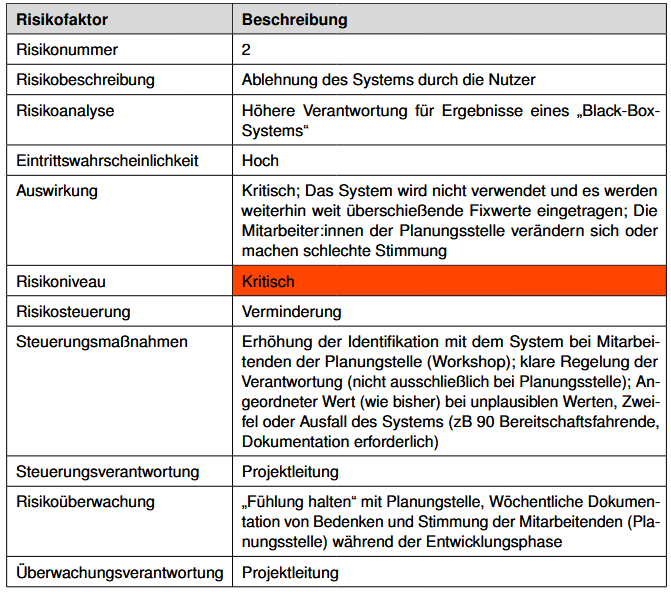
\includegraphics[width=15cm]{01_resources/risk2.png}\\
Quelle: \cite{grunsky_rettungsdienst_2025}
\label{fig:risk2}
\end{figure}
\FloatBarrier 


\section{Learnings}
\label{learned}

Durch die Umsetzung dieses Projektes von der Use Case Analyse über die Projektplanung bis hin zu einer ersten Entwicklung konnte ein tieferes Verständnis für das Zusammenspiel bestehender Werkzeuge, die Bedeutung von Schnittstellen und Struktur in der Arbeit mit diesen Werkzeugen aber auch die Unzulänglichkeiten mit der Prozesse und Frameworks teils spezifiziert sind, erlangt werden. 

Speziell auf die Entwicklung der Modelle bezogen, erweiterte die Arbeit mit Machine Learning Frameworks in R wie \textit{caret} \citep{kuhn_caret_2019} und \textit{fpp3} \citep{hyndman_forecasting_2021}, aber auch mit Werkzeugen wie Quarto \citep{posit_quarto_2025} das eigene Repertoire der Entwicklung und half dabei eine eigene Vorlage und Arbeitsweise für zukünftige Projekte anzulegen.

Nächste Schritte in diesem Projekt sollten 

\begin{itemize}
 \itemsep-8pt
 \item eine Diskussion mit dem Präsidium über die Definition einer fallspezifischen Kostenfunktion,
 \item das Finetuning von Hyperparametern, sowie
 \item die Umsetzung eines modell- und geschäftszentrierten Monitorings der Vorhersagemodelle 
\end{itemize}

enthalten.








